\documentclass[]{scrartcl}

\usepackage{amsmath}
\usepackage{amssymb}
\usepackage[utf8]{inputenc}
\usepackage[T1]{fontenc}
\usepackage{lmodern}
\usepackage{ngerman}
\usepackage{geometry}
\usepackage{graphicx}
\usepackage{wrapfig}
\usepackage{caption}
\usepackage{wasysym}
\usepackage{siunitx}
\usepackage{picinpar}
\usepackage{tikz}
\usepackage{float}

\renewcommand{\figurename}{Abb.}
\usepackage[
	colorlinks=true,
	urlcolor=blue,
	linkcolor=black
]{hyperref}


%Hier Titel und so
\newcommand{\versuchnummer}{V49} 
\newcommand{\versuchname}{Messung von Diffusionskonstanten mittels gepulster Kernspinresonanz} 
\newcommand{\versuchdatum}{11.01.2016} 


\title{Versuch \versuchnummer\\ \versuchname}
\subtitle{Physikalisches Fortgeschrittenenpraktikum}
\author{Robert Rauter und Björn Lindhauer}
\date{\versuchdatum} 
\begin{document}
\begin{titlepage}
{\large \versuchdatum}
\vspace{7cm}
\begin{center}
\textbf{\huge Versuch \versuchnummer}\\
\vspace{0.5cm}
\textbf{\huge \versuchname}\\
\vspace{0.2cm}
\textbf{ Physikalisches Fortgeschrittenenpraktikum}\\
\vspace{9cm}

{\Large Robert Rauter \ \ \hspace{1.5cm} und \hspace{1.5cm} Björn Lindhauer}\\
{ \url{robert.rauter@tu-dortmund.de} \ \ \hspace{2cm} \url{bjoern.lindhauer@tu-dortmund.de}}
\end{center}
\end{titlepage}
\section{Einleitung}
Die Grundlage der Kernspinresonanz ist, dass sich magnetische Momente der Atomkerne beim wirken eines äußerem Magnetfeld ausrichten. Die Ausrichtung kann durch Einstrahlung von Hochfrequenzquanten mit geeigneter Frequenz verändert werden und so können verschiedene magnetische Eigenschaften einer Probe untersucht werden.\\
Zum einen können Resonanzphänomene beobachtet werden, indem die Energieaufnahme in Abhängigkeit der Frequenz aufgenommen wird. So lassen sich Rückschlüsse auf lokale Magnetfelder anhand der Resonanzstellen schließen. Mit diesen Daten kann die Struktur der Probe rekonstruiert werden.\\
Zum anderen kann der zeitlicher Verlauf von Auf- und Abbau eines Magnetfeldes bestimmt werden. Außerdem lässt sich die Diffusionskonstante einer Probe bestimmen, da sich durch die Diffusion die Anzahl der Momente im Messabschnitt ändert und folglich das statische Magnetfeld der Probe verändert ist. Die Resonanzbedingung ändert sich und aus dieser Änderung lässt sich die Diffusionskonstante bestimmen. Da Resonanzbedingung erfüllt werden sollen, werden Hochfrequenzimpulse benötigt, welches dieser Methode ihren Namen gepulste Kernspinresonanz gab.\\
In diesen Versuch soll mit der gepulsten Kernspinresonanz eine Probe untersucht werden.
\section{Theoretische Grundlagen}
\subsection{Magnetisierung}
Zunächst wird angenommen, dass die Probe im thermischen Gleichgewicht mit der Umgebung steht, da Konvektionsströme nicht Bestandteil der Betrachtungen sind.\\
Des weiteren sei ein homogenes Magnetfeld $B_0\ \vec{e_z}$ angelegt.\\
Durch dieses Feld spalten die entarteten Kernspinzustände
Magnetisierung einer Probe, die im thermischen Gleichgewicht mit der Umgebung steht mit der Spinquantenzahl $I$ in $2I+1$ äquidistante Unterniveaus auf, welche den Abstand $\Delta E = \gamma B_0 \hbar$ besitzen.\\
Die Besetzung der Niveaus erfolgt nach der Boltzmann-Verteilung. Es folgt daraus das Besetzungszahlverhältnis 
\begin{align}
\frac{N\left(m\right)}{N\left(m-1\right)}=\exp \left(-\frac{\gamma B_0\hbar}{k_\text{B}T}\right)
\end{align}
bei gegebenen $T$.\\
Da die Besetzung folglich nicht homogen über alle Zustände ist, besitzt der Kern eine Kernspinpolarisation
\begin{align}
\left\langle I_Z \right\rangle = \frac{\sum\limits_{m=-I}^{I} \hbar m \exp\left(-\beta m\gamma B_0 \hbar \right)}{\sum\limits_{m=-I}^{I} \exp\left(-\beta m\gamma B_0 \hbar \right)} \label{eq_izallgemein}\hspace*{0.5cm}\text{.}
\end{align}
Im folgenden werden nur noch Protonen betrachtet, es ist somit $I=\frac{1}{2}$. Ein Niveau spaltet sich in zwei Unterniveaus auf mit den Quantenzahlen $m=-\frac{1}{2}$ und $m=+\frac{1}{2}$. Abbildung \ref{fig_aufspaltung} veranschaulicht dies.
\begin{figure}[H]
\centering
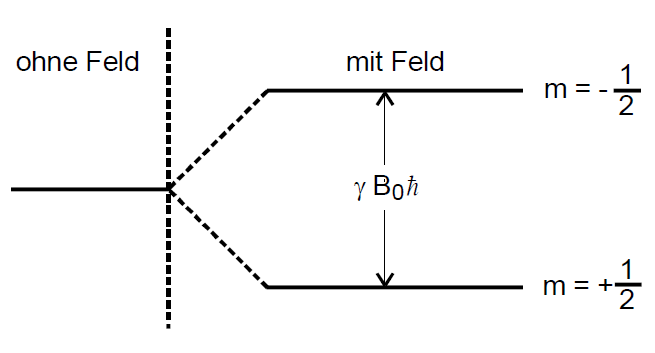
\includegraphics[width=8cm]{images/aufspaltung_magnetfeld.png}
\caption{Toller Titel (1)}
\label{fig_aufspaltung}
\end{figure}
Für die Exponentialfunktion in \ref{eq_izallgemein} kann eine lineare Näherung eingesetzt werden, falls
\begin{align}
m\gamma B_0 \hbar \ll k_\text{B}T 
\end{align}
ist, welches für Magnetfelder in der Größenordnung von 1 Tesla und Temperaturen nahe der Zimmertemperatur gegeben ist.\\
Es ergibt sich
\begin{align}
\left\langle I_Z \right\rangle_{\text{P}}= -\frac{\hbar^2}{4}\frac{\gamma B_0}{k_\text{B}T}\hspace*{0.5cm}\text{.} \label{eq_iznahrung}
\end{align}
Da die Kernspinpolarisation im direkten Zusammenhang mit den magnetischen Momenten $\vec{\mu}_I$ stehen, ist eine makroskopische Magnetisierung $\vec{M_0}$ der Probe messbar, die durch die Summe aller Einzelmomente pro Volumen
\begin{align}
\vec{M_0}=\sum\limits_{i}^{}\frac{\mu_0\vec{\mu}_i}{V}
\end{align}
gegeben ist.\\
Es ist
\begin{align}
\left\langle \vec{M_0}_z \right\rangle =N\gamma \mu_0 \left\langle I_Z \right\rangle_{\text{P}} :=\left\langle M_0 \right\rangle\hspace*{0.5cm}\text{.}
\end{align}
Wird nun \ref{eq_iznahrung} eingesetzt, so ergibt sich
\begin{align}
\left\langle M_0 \right\rangle = N\frac{\hbar^2}{4}\mu_0\frac{\gamma^2 B_0}{k_\text{B}T}:=M_0
\end{align}
als Gleichgewichtsmagnetisierung bei Temperatur $T$.
\subsection{Larmor-Präzession}
Damit das System interessantes Verhalten zeigt, muss $\vec{M}$ aus der Gleichgewichtslage $\vec{M_0}$ durch Hochfrequenzquanten mit Energie $\Delta E$ gebracht werden.\\
Außerdem kann das System klassisch betrachtet werden, da die Magnetisierung durch $N$ Spins mit $N \sim 10^{28}$ m$^{-2}$ erzeugt werden und folglich Quanteneffekte nicht relevant sind.\\
Es wirkt somit ein Drehmoment
\begin{align}
\vec{D}=\vec{M}\times B_0 \vec{e_z}
\end{align}
und es lässt sich dadurch über die Kreiselgleichung die Differenzialgleichung
\begin{align}
\frac{d \vec{M}}{d t} = \gamma \vec{M}\times B_0 \vec{e_z}\label{eq::magzeit}
\end{align}
herleiten.\\
Die komponentenweise Lösung der Differenzialgleichung ist durch
\begin{align}
M_x&= 0 \\
M_y&= A \cos \gamma B_0 t \\
M_z&= -A \sin \gamma B_0 t
\end{align}
gegeben.\\
Es folgt eine Präzession um $\vec{e_z}$-Achse mit der Larmor-Frequenz genannten Frequenz
\begin{align}
\omega_L =\gamma B_0 \hspace*{0.5cm}\text{.}
\end{align}
\subsection{Relaxationserscheinungen}
Der zeitliche Verlauf der Magnetisierung ist durch die Blochschen Gleichungen gegeben, die eine Zusammensetzung aus der Kreiselgleichung und der Differentialgleichung für die Relaxion besteht.\\
In diesen Fall lauten sie
\begin{align}
\frac{d M_x}{d t}&= \gamma B_0 M_y - \frac{M_x}{T_2}\\
\frac{d M_y}{d t}&= \gamma B_0 M_x - \frac{M_y}{T_2}\\
\frac{d M_z}{d t}&= \frac{M_0-M_Z}{T_1}\hspace*{0.5cm}\text{.}
\end{align}
Es wurden dabei zwei Zeitkonstanten $T_1$ und $T_2$ eingeführt.\\
$T_1$ longitudinale oder Spin-Gitter-Relaxationszeit:
- Veränderung der Magnetisierungskomponente parallel zur Feldrichtung $\vec{B_0}$ 
- Energie aus dem Kernspinsystem zu Gitterschwingungen
$T_2$ transversale Spin-Spin-Relaxationszeit
-Abnahme der Magnetisierung senkrecht häufig durch Spin-Spin-Wechselwirkungen
\subsection{HF-Einstrahlungsvorgänge}
Hochfrequenzfeld mit Magnetfeld $\vec{B_1} \perp \vec{e_z}$
Feld gegeben durch
\begin{align}
\vec{B_{\text{HF}}}=2\vec{B_1} \cos \omega t
\end{align}
Aufteilbar in zwei zirkular polarisierte Felder $\omega_+$ und $\omega_-$
Wenn $\omega_+$ nahe Larmor-Frequenz --> $\omega_-$ irrelevant
--> rotierendes Feld um $\vec{e_x}$ und $\vec{e_y}$-Achse
--> Wirkt gesamtes Magnetfeld auf Probe
\begin{align*}
B_x=B_1 \cos \omega t \\
B_y=B_1 \sin \omega t \\
B_z=B_0
\end{align*}
Sinnvoll: Transformation Koordinatensystem mit Zeitabhängigen Einheitsvektoren mit
\begin{align}
\frac{\partial \vec{\tilde{e_x}}}{\partial t}= -\vec{\omega} \times \vec{e_x}\\
\frac{\partial \vec{\tilde{e_y}}}{\partial t}= -\vec{\omega} \times \vec{e_y}\\
\frac{\partial \vec{\tilde{e_z}}}{\partial t}= 0
\end{align}
Lösung DGL 
--> 
\begin{align}
\frac{d \vec{M}}{d t}= \gamma \vec{M}\times \left(\vec{B}_{\text{ges}}+\frac{\vec{\omega}}{\gamma}\right)
\end{align}
--> Gleichung \ref{eq::magzeit} mit effektiven Magnetfeld
\begin{align}
\vec{B}_\text{eff}=\vec{B}_0+\vec{B}_1+\frac{\vec{\omega}}{\gamma}
\end{align}
--> Analog zu Vorherigen Abschnitt --> Präzessionsbewegung um Feldrichtung von $B_{\text{eff}}$
--> Wichtiger Fall: Resonanz $\omega=\omega_L$ --> $\vec{B}_{\text{eff}}=\vec{B}_1$
präzediert um $\vec{B}_1$-Achse --> Präzessionskegel $90^\circ$
Drehwinkel $\delta\left(\delta t\right)$ berechenbar
\begin{align}
\delta\left(\Delta t\right)=\gamma B_1 \Delta t
\end{align}
Einstrahlzeit:
$\Delta t_{90}=\frac{\pi}{2\gamma B_1} $
Es ist $\Delta t_{90} \ll T_1,T_2$
Dabei wird $\vec{M}$ von der $-\vec{e_z}$ Richtung in die  $\vec{e_y}$ gedreht.
Analog $\Delta t_{180}$ Dabei wird $\vec{M}$ von der $\vec{e_z}$ Richtung in die  $-\vec{e_z}$ gedreht. 
Wenn Magnetisierung wieder in die Ruhelage --> $T_1$ und $T_2$ bestimmbar

\section{Durchführung}


\section{Quellen}

\end{document}